\section{Formal Semantics}\label{sec:formal}
\marco{Old notes: new text is later}
Yanlin and Haoyuan

We need to show 2 things:

1) The dynamic semantics: what's the code that gets generated by a mixin annotation;

2) The type system: what programs to reject; properties: generation of type-safe/checkable code.

\bruno{The implementation is still missing the type system (rejecting some
  programs)!}

\bruno{Some notes for discussion regarding formalization:
\begin{itemize}
\item Syntax and Rules:
We can make it more compact and consistent by use overline
notation more, instead of \ldots.
\item Order of premisses: It may be worthwhile to swap the order of
some premisses, so that it follows the order of the explanations.
\item T-Invk: I think we need to type-check $e_0$ separately. Otherwise
$C_0$ shows up magically.
\item T-Obj: small fixes on 3rd line. Suggestion, create two
auxiliary functions: $sigvalid(C,\overline{mh})$ and $alldefined(C,\overline{mh})$
\item T-INTF: $C_0$ is $I$. Type of this was $C$, modified it to $C_0$.
In the last line, should it be $dom(\overline{meth})$ or just $\overline{meth}$?

\item tops and shadow: tops seems redundant;
we use tops to collect classes, so just that in the next step we iterate
over those classes to collect methods that satisfy some property.
I think we can merge those 2 steps.

\item I have trouble following the definition of shadow; I think there
are errors there.

\end{itemize}
}

\footnote{Future work: updating multiple fields in one method call,
  \texttt{with(T v)}}



\begin{figure}[h]
\begin{grammar}
\production{
\e
}{
  \x\mid\MCall\e\m\es\mid\MCall{\C}\m\es\mid\MCall{\C\QM{.super}}\m\es\mid\obj
  }{expressions}\\
\production{
\obj
}{
\QM{new}\ \C\oR\cR\oC\fields\
\mh_1\oC\QM{return}\ \e_1\QM{;}\!\cC
\ldots
\mh_n\oC\QM{return}\ \e_n\QM{;}\!\cC
\cC
  }{object creation}\\
\production{\field}{\T\ \f \QM= \x\QM;}{field declaration}\\
\production{
\II
}{
 \ann\ \QM{interface}\ \C_0\ \QM{extends}\ \Cs\ \oC\ \methods\ \cC
  }{interface declaration}\\
\production{
\method
}{
 \QM{static}\ \mh\ \oC\QM{return}\ \e\QM{;}\!\cC
\mid
\QM{default}\ \mh\oC\QM{return}\ \e\QM{;}\cC
\mid
\mh\QM{;}
  }{method declaration}\\
\production{
\mh
}{
 \T_0\ \m\ \oR\T_1\ \x_1\ldots\T_n\ \x_n\cR
  }{method header}\\
\production{
\ann
}{
  \mixinAnn|\emptyset
  }{annotations}\\
\production{\Gamma}{
\x_1{:}\C_1\ldots\x_n{:}\C_n
}{environment}
\end{grammar}
\caption{Grammar of ClassLess Java}
\label{Grammar}
\end{figure}

${}_{}$\\
\begin{figure}[h]
$
\!\!\!\!\!\!\!\!\!\!
\begin{array}{l}
\inferrule[(T-Invk)]{
 \Gamma \vdash \e_0 \in \C_0 \\\\
\forall i\in 1..n\  \Gamma \vdash \e_i \in \_<:\C_i \\\\
  \textsf{mtype}(\m,\C_0) \!=\! \C_1\ldots\C_n \!\!\to\! \C
%\textsf{mmodifier}(\m,\C_0) \neq \textbf{static}
 }{
 \Gamma \vdash \e_0\QM.\m\QM(\e_1\ldots\e_n\QM) \in \C }
\quad
\inferrule[(T-StaticInvk)]{
\forall i\in 1..n\  \Gamma \vdash \e_i\in \_<:\C_i \\\\
\textsf{mtypeS}(\m,\C_0) \!=\! \C_1\ldots\C_n \!\!\to\! \C
%\textsf{mmodifier}(\m,\C_0) = \textbf{static}
}{
\Gamma \vdash \C_0\QM.\m\QM(\e_1\ldots\e_n\QM) \in \C}
\quad
\inferrule[(T-SuperInvk)]{
\Gamma(\this) <: \C_0 \\\\
\forall i\in 1..n\ \Gamma \vdash \e_i\in \_<:\C_i \\\\
  \textsf{mtype}(\m,\C_0) \!=\! \C_1\ldots\C_n \!\!\to\! \C
%\textsf{mmodifier}(\m,\C_0) \neq \textbf{static} \\\\
}{\Gamma \vdash \C_0\QM.\QM{super}\QM.\m\QM(\e_1\ldots\e_n\QM) \in \C}

\\[5ex]
\inferrule[(T-Obj)]{
\forall i\in 1..n\
%\Gamma_i
\Gamma,\f_1{:}\T_1,\ldots,\f_k{:}\T_k,\,\QM{this}{:}\C,\Gamma^{\mh_i}
\vdash\e_i\in \_\subtype\C^{\mh_i}\\\\
\forall i\in 1..n\ \mh_i\subtype\mBody(\m^{\mh_i},\C)\\\\
\forall i\in 1..k\ \Gamma(\x_i)\subtype\T_i\\\\
\forall\m\mbox{ such that }
\mBody(\m,\C)=\mh\QM; \exists i\in 1..n\ \m^{\mh_i}=\m
%\forall i\in 1\ldots n\ \Gamma_i=\Gamma,\f_1{:}\T_1,\ldots,\f_k{:}\T_k,\,\QM{this}{:}\C,\Gamma^{\mh_i}
}{
\Gamma \vdash\QM{new}\ \C\oR\cR\oC\T_1\ \f_1\QM=\x_1\QM;\ldots\T_k\ \f_k\QM=\x_k\QM;\
\mh_1\oC\QM{return}\ \e_1\QM{;}\!\cC
\ldots
\mh_n\oC\QM{return}\ \e_n\QM{;}\!\cC
\cC
\in\C
}
\quad
\inferrule[(T-Var)]{
\Gamma(\x)=\C
}{
\Gamma \vdash x \in\C}
\\[5ex]
 \inferrule[(T-Intf)]{
IT(\C_0) = \ann\ \QM{interface}\ \C_0\ \QM{extends}\ \C_1\ldots\C_n \oC\methods\cC\\\\
 \forall \QM{default}\ \mh\oC\QM{return}\ \e\QM;\cC \in \methods,
\ \Gamma^{\mh},\,\QM{this}{:}\C_0\vdash\e\in \_\subtype\C^{\mh} \\\\
 \forall \QM{static}\ \mh\oC\QM{return}\ \e\QM;\cC \in \methods,
\ \Gamma^{\mh}\vdash\e\in \_\subtype\C^{\mh} \\\\
\dom(\C_0)=\dom(\C_1)\cup\ldots\cup\dom(\C_n)\cup\dom(\methods)
 }{
\C_0 \text{ OK}
}
\end{array}$
\caption{Typing}
\label{ET}
\end{figure}
\subsection{Grammar and typing rules}${}_{}$\\



In Figure~\ref{Grammar} we show the syntax of ClassLess Java.%
\footnote{To be compatible with java, the concrete syntax for an interface declaration with empty supertype list $\C_1\ldots\C_n$ would also omit the \Q@extends@ keyword.}

We formalize a minimal version of Java 8, focusing on Interfaces, default methods and object creation literals.
As you can see, we have no syntax for classes.
Expressions are the conventional variable and method call$\x$ and$\e\QM.\m\QM(\es)$, then we have conventional static method call
$\C\QM.\m\QM(\es)$; for simplicity we do not consider the degenerate case of calling a static method over the this receiver as it considered a bad/confusing programming practice.
Next we have the more interesting super call $\C\QM{.super.}\m\QM(\es)$, whose semantic is to call the (non static) method $\m$ over the $\this$ receiver, but statically dispatching to the version of the method defined in the interface $\C$.
Finally, we consider the object initialization expression from an interface $\C$, where (for simplicity) all the fields are initialized with a variable present in scope.
Note how our language is exactly a subset of Java 8.
We allows the only annotation \mixin since is the only one interesting in this article.
We consider an globally present Interface Table (\metaVar{IT}) mapping from interface names $\C$ to interface declarations \metaVar{I}.

The environment $\Gamma$ is a mapping from variables to types.
As tradition, we allows functional notation for $\Gamma$.
However, to help us defining auxiliary functions,
we also allows functional notation set of methods $\methods$, using the method name $\m$ as a key.
That is, we define $\methods(\m)=\method$ iff there is a unique $\method\in\methods$ whose name is $\m$.
For convenience, we define $\methods(\m)=\none$ otherwise;
moreover $\m\in\dom(\methods)\ \miff\ \methods(\m)=\method$.

 Typing statement $\Gamma \vdash \e\in\C$ reads ``in the
environment $\Gamma$, expression $\e$ has type $\C$.''
As a shortcut, we write $\Gamma \vdash \e\in\C<:\C'$
instead of $\Gamma \vdash \e\in\C$ and $\C<:\C'$.
 From the interface table, we can read off the subtype relation between interfaces. The subtype relation is given by the \textbf{extends} clauses in the interfaces. We omit the definition of the usual, traditional subtyping relation between interfaces.%
\footnote{
Notice how there are no classes, thus there is no subclassing.
We believe that this approach may scratch an old itching point in the long struggle of subtyping versus subclassing:
According to some authors, from a software engineering perspective, interfaces are just a kind of classes. Others consider more opportune to  consider interfaces are pure types. In this vision our language would have no subclassing. We do not know how to conciliate those two viewpoints and ClassLess Java design. We do not have Classes purely in the Java sense.
}

In Figure~\ref{ET} we show the typing rules.
We use the following auxiliary notation:
$\Gamma^\mh$ trivially extract the environment from a method header, collect the types and the names of the method parameters.
$\m^\mh$ and $\C^\mh$ extracts the method name and the return type from a method header.
$\mBody(\m,\C)$ return the full method declaration as seen by $\C$, that is the method $\m$ can be declared in $\C$ or inherited from another interface.
$\mBody(\m,\C)$ will be formally defined later.
$\textsf{mtype}(\m,\C)$ and
$\textsf{mtypeS}(\m,\C)$ return the type signature from a method (using $\mBody(\m,\C)$ internally).
$\textsf{mtype}(\m,\C)$ is defined only for non static methods, while
$\textsf{mtypeS}(\m,\C)$ only on static ones.

We use $\dom(\C)$ to denote the set of methods that are defined for type $\C$, that is: $\m\in\dom(\C)\ \miff \ \mBody(\m,\C)=\method$.

We discuss first the most interesting rules, that is
\rn{(t-Obj)} and  \rn{(t-Intf)} \marco{Bruno, you can explain t-obj, if you can make it understandable, I go for t-inft}

Rule \rn{(t-Obj)}....

Rule \rn{(t-intf)} check that an interface $\C_0$ is correctly typed.
First we check that the body of all the default and static methods are well typed.
Then we check that
$\dom(\C_0)$ is the same of $\dom(\C_1)\cup\ldots\cup\dom(\C_n)\cup\dom(\methods)$.
This is not a trivial check, since $\dom(\C)$ is defined using $\mBody$, that is undefined in many cases: notably if a method $\method\in\methods$ is not compatible with some method in
$\dom(\C_1)\ldots\dom(\C_n)$ or if any method in both $\dom(\C_i)$ and $\dom(\C_j)$ ($i,j\in 1..n$)  is conflicting.

\marco{if we have space we can discuss the other rules too, but is not mandatory}




\subsection{Auxiliary Definitions}

\begin{comment}
\subsubsection{Auxiliary function: \textsf{mtype}}
- \textsf{mtype(m, C)} : the signature of method m in C.

\[ \inferrule{
  IT(T) = \text{\emph{ann} interface } C \{ \overline{M} \} \\
  E \spc m(\overline{D} \spc \overline{x}) \{ \text{return } e; \} \in M}
{ \textsf{mtype(m,T)} = \overline{D} \to E } \]

\[ \inferrule{
  IT(T) = \text{\emph{ann} interface } C \{ \overline{M} \} \\
  m \notin M}
{ \textsf{mtype(m,T)} = \emptyset } \]

\[ \inferrule{
  IT(T) = \text{\emph{ann} interface } C \text{ extends } C_1,...,C_k \{ \overline{M} \} \\
  E \spc m(\overline{D} \spc \overline{x}) \{ \text{return } e; \} \in M}
{ \textsf{mtype(m,T)} = \overline{D} \to E } \]

\[ \inferrule{
  IT(T) = \text{\emph{ann} interface } C_0 \text{ extends } \overline{C} \{
  \overline{M} \} \\
  m \notin M}
{ \textsf{mtype(m,T)} = \bigcup \textsf{mtype}(m,\overline{D}) } \]
\end{comment}


Defining \mBody{} is not trivial, and requires quite a lot of attention to the specific model of Java Interfaces, and on how it differs w.r.t. Java Class model.
$\mBody(\m,\C)$ denotes the actual body of method $\m$ that interface $\C$ owns. It can either be defined originally in $\C$ or in its supertypes, and then passed to $\C$ via inheritance.

The body of a method $\m$ contains all the relevant information with respect to that method, like the type of $\m$ as well as the modifier.
We use internally a special modifier $\conflicted$ to denote the case of two methods with conflicting implementation.\\*

$\mBody(\m,\C_0) = \override(\methods(\m),
\shadow(\m,\Aux{tops}(\Cs)))
$\\*
Where
$\metaVar{IT}(C_0) =
\ \ann\ \QM{interface}\ \C_0\ \QM{extends}\ \Cs \oC\methods\cC$

As you can see, we are delegating the work to three others auxiliary functions: $\tops(\Cs), \shadow(\m,\Cs) and \override(\method,\method')$
${}_{}$\\*
\marco{we need to discuss the names tops, shadow and override}

\tops{} recover from the interface table only the ``needed'' methods, that is, 
the non static ones that are not transitively reachable by following another, less specific, superinterface chain. Formally:\\*
$\method\in\tops(\m,\Cs) \mbox{ iff }\C\in\Cs\ ,\method=\mBody(\m,\C), \method\mbox{ not a static method}$\\*
${}_{}$\tab and $\nexists \C'\in\Cs\setminus\C$ such that $\C' \subtype \C$.

\shadow{} choose the most specific version of a method, that is the unique version available, or a conflicted version from a set of possibilities.
We do not model overloading, so it is an error if multiple versions are available with different parameter types. Formally:\\*
\!\!\!\!$\begin{array}{l}
%\shadow(\m,\C_1\ldots\C_n)=\shadow(\methods)
%\whereNote
% \mwhere\ \mBody(\m,\C_i)\in\methods
%\ \mif\ \mBody(\m,\C_i)\in\{\mh\QM;,\QM{default}\ \mh\mbox{\Q@\{return \_;\}@}\}
%\\ &\mor\ \mBody(\m,\C)=\mh\QM;
%\\

\shadow()=\none\\
\shadow(\method)=\method\\
\shadow(\overline{\mh\QM;})=\Aux{mostSpecific}(\overline{\mh\QM;})\\
\shadow(\methods)=\conflicted\mh\QM;
\whereNote
\mwhere\ 
\methods\mbox{ not of the form }\overline{\mh\QM;}\mbox{ and }
\Aux{mostSpecific}(\methods)\in\{\mh\QM;,\QM{default}\ \mh\mbox{\Q@\{return \_;\}@}\}\\
\Aux{mostSpecific}(\methods)=\method
\whereNote
\mwhere\ \method \in \methods\ \mand\ \forall \method' \in \methods :  \method \subtype
                                       \method', \\
\T\ \m\oR\T_1\x_1\ldots \T_n\x_n\cR \subtype \T' \m\oR\T_1\x_1'\ldots\T_n\x_n'\cR
\whereNote
 \mwhere\ \T\subtype \T'\\

\method \subtype
\QM{default}\ \mh\mbox{\Q@\{return \_;\}@}=
\method\subtype\mh\QM;
\\
\QM{default}\ \mh\mbox{\Q@\{return \_;\}@}\subtype\method=
\mh\QM;\subtype\method
\end{array}$
${}_{}$\\*
Where $\Aux{mostSpecific}$ return the most specific method using return type specialization as introduced in Java ??
We just check the subtype between method headers, so we discard information abut method implementation.\\*
${}_{}$\\*
The override function models how the implementation in an interface can override implementation in the superinterface; even in case of a conflict.
Note how we use the special value $\none$, and how (forth case) overriding can solve a conflict.
\\*
\!\!\!\!$\begin{array}{ll}
\override(\none,\none)=\none\\
\override(\method,\none)=\method\\

\override(\none,\method)=\method
\whereNote
\mwhere\ \method\mbox{ not of the form } \conflicted\ \mh\QM;\\
\override(\method,\method')
=
\method
\whereNote
\mwhere\ \method'\in\{\mh\QM;,\QM{default}\ \mh\mbox{\Q@\{return \_;\}@}, \conflicted\ \mh\QM; \},
\method\subtype\method'
\\
%\override(\method,\mh')
%=\method
%\whereNote
%\mif\ \method\in\{\mh\QM;,\QM{default}\ \mh\mbox{\Q@\{return \_;\}@} \}, \mh\subtype\mh'
%\override(\_,\_)=\error & Otherwise
%\textsf{shadow}(body_1, body_2)=\emptyset & \textsf{if }body_1.\textsf{modifier}=body_2.\textsf{modifier}=\textbf{static}\\
%\textsf{shadow}(body_1, body_2)=body_1 & \textsf{if }body_2=\emptyset\textsf{ or }body_2.\textsf{modifier}=\textbf{static}\\
%\textsf{shadow}(body_1, body_2)=body_2 \hspace{.1in}  & \textsf{if }body_1=\emptyset\textsf{ or }body_1.\textsf{modifier}=\textbf{static}
\end{array}$


\begin{figure}[tbp]
\centering
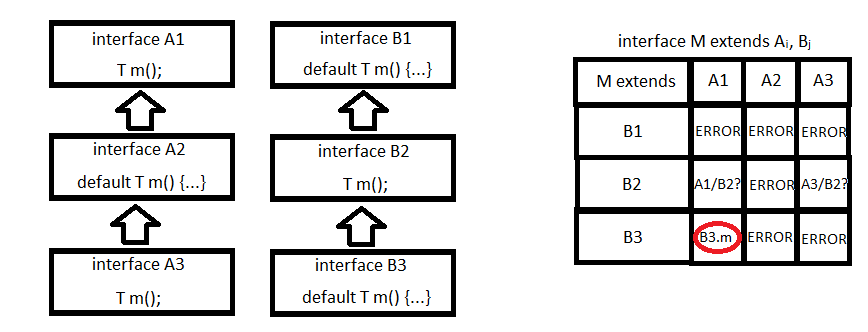
\includegraphics[width=5in]{table.png}
\caption{Table.}\label{table_png}
\end{figure}

%The \textsf{shadow} function takes two same methods (with the same name and types of arguments), and return the method which shadows the other during inheritance.
%exmples to motivate our design
%interface A{static String m(){return "A";}}
%interface C extends A{
%	default String dm(){
%		  this.m();//wrong in java
%		  A.m();
%		  C.m();//wrong in java
%		}
%}
%
%
%(1) Static methods are not inherited. Also, if one of $\{body_1,body_2\}$ is null, \textsf{shadow} simply returns the other one. Hence

\begin{comment}
%Now it is correct, but may be we do not need it?
We abbreviate typing statements on
sequences in a simple way, writing $\Gamma \vdash \overline{t}:\overline{C}$ as
shorthand for $\Gamma \vdash t_1:C_1,..., \Gamma \vdash t_n:C_n$.
\end{comment}

\marco{The notation mtype get only non static methods, the notation mtypeS get only static ones}

%\subsubsection{Interface and method Typing}





\begin{comment}
\subsubsection{Method Typing}


\[
\inferrule
{ }
{T_0 \spc m(\overline{T} \spc \overline{x}); \text{ OK IN I} }
\quad \textsc{(T-Meth)}
\]

\[
\inferrule
{\overline{x}:\overline{T} \vdash e:S \\ S <: T_0}
{T_0 \spc m(\overline{T} \spc \overline{x}) \text{ \{ return } e;\} \text{ OK IN
    I} \\\\ \Gamma \vdash \textbf{this}:I }
\quad \textsc{(T-MethBody)}
\]

\[
\inferrule
{IT(I)=\text{interface } I \text{ extends } \overline{J} \text{\{...\}} \\
\forall i,\text{if \textsf{mtype}}(m,J_i) = \overline(T) \to U_0, \text{then }
T_0 <: U_0 }
{T_0 \spc m(\overline{T} \spc \overline{x}); \text{ OK IN I} }
\quad \textsc{(T-MethExt)}
\]

\[
\inferrule
{\textbf{this}:I, \overline{x}:\overline{T} \vdash e:S \\ S <: T_0 \\\\
IT(I)=\text{interface } I \text{ extends } \overline{J} \text{\{...\}} \\\\
\forall i,\text{if \textsf{mtype}}(m,J_i) = \overline(T) \to U_0, \text{then }
T_0 <: U_0 }
{T_0 \spc m(\overline{T} \spc \overline{x}) \text{ \{ return } e;\} \text{ OK IN
    I} }
\quad \textsc{(T-MethBodyExt)}
\]

\[ \inferrule
{\textbf{interface } I \textbf{ extends } \overline{J} \{ \overline{M} \} \\\\
 \forall J_i \in \overline{J}, J_i \text{ OK} \\\\
 \forall m \in \overline{M}, \textsf{mbody}(m,I) \neq \error \\\\
 \forall J_i \in \overline{J}, \forall m \text{ inside } J_i,
 \textsf{mbody}(m,I) \neq \error }
{I \text{ OK}}
\quad \textsc{(T-Intf)}
 \]

Interface $I$ type checks well, if:
\begin{itemize}
\item All its super-interfaces $\overline{J}$ OK.
\item All methods inside interface $I$ are OK.
\item All methods that $I$ is inheriting from super-interfaces are OK.
\end{itemize}
\subsubsection{Subtyping}

\[ \inferrule{}{T <: T} \]

\[ \inferrule{S <: T \\ T <: U}{S <: U}\]

\[ \inferrule{\emph{ann} \spc \textbf{interface} \spc C_0 \spc \textbf{extends} \spc C_1,...,C_k \{...\}}
{C_0 <: C_1 \\ ... \\ C_0 <: C_k} \]
\end{comment}
%\subsubsection{Interface Table}






\subsection{What  \mixin Generates}
We now show what the \mixin annotation generates. We present a formal definition for
most of the generated methods; however in our formalism we do not consider setters, so we do not formally define the generation of the setters. 
We do not include casts or \Q@instanceof@, so we do not include the \Q@with@ method.

\subsubsection{Translation Function}${}_{}$\\*

\noindent$[\![\mixinAnn\ \QM{interface}\ \C_0\ \QM{extends}\ \Cs \oC \methods \cC ]\!] =
\emptyset\ \QM{interface}\ \C_0\ \QM{extends}\ \Cs\ \oC 
\methods\ \methods' \cC
$\\*${}_{}$\tab
where  $\valid(\C_0)$,\Q@of@$\notin\dom(\methods)$ and $\methods'=\ofMethod(\C_0) \ \otherMethod(\C_0,\methods)$.\\*

To translate an annotated interface, we add the \Q@of@ method, and then we add some other methods.
However, first of all we check if the interface is valid for annotation:

\noindent$\valid(\C_0)$  holds if $\forall \m\in\dom(\C_0),$ if $\mh\QM; = \mBody(\m, \C_0),$ one case is satisfied:
$\isField(\method)$,
$\isWith(\method, \C_0)$
or $\isClone(\method, \C_0)$.

That is, we can categorize all the \emph{not implemented} methods in a pattern that we know how to implement.
To complete our formal definition we would need to add setters and \Q@with@.
Moreover, we check that the method \Q@of@ is not already defined by the user.
In our simplified formalization we consider this to be just an error.
In our prototype we keep \Q@overloading@ into account, and so we check that an of method with the same signature of the one we would like to generate is not already present.\marco{Do we check it?}


In the following we will write $\QM{with#}\m$ to append $\m$ to \QM{with}, following the camelCase rule, so the first letter of
$\m$ must be lower-case and is turned in upper-case upon merging.
For example \QM{with#foo}=\QM{withFoo}.
Special names $\specialName(\m)$ are \QM{clone}, \QM{with} and all the identifiers of form $\QM{with#}\m$.

\subsubsection{$\ofMethod$}${}_{}$\\*
We now formally define $\ofMethod$, the function that generates the method \QM{of}, that behaves like a factory. To avoid boring digressions about well known ways to find unique names, for the sake of this formalization we assume that all the methods do not start with underscore, and we prefix method names with underscore to obtain valid  parameter names.\\*
\noindent$\begin{array}{l}
\ofMethod(\C_0) = \
 \QM{static}\ C_0\ \QM{of} \oR \C_1\ \QM_\m_1\QM,\ldots \C_n\ \QM_\m_n\cR\
\QM{\{}
\QM{return new}\ C_0 \oR\cR\ \QM{\{} \\
\tab\tab\tab\tab\tab\tab\tab C_1\ \m_1 = \QM_\m_1\QM;\ldots \C_n\ \m_n = \QM_\m_n\QM; \\
\tab\tab\tab\tab\tab\tab\tab
\C_1\ \m_1\oR\cR\ \QM{\{return }\ \m_1\QM{;\}}\ \ldots 
\C_n\ \m_n\oR\cR\ \QM{\{return }\ \m_n\QM{;\}}\\
\tab\tab\tab\tab\tab\tab\tab\withMethod(\m_1,\C_0,\es_1)\ldots\withMethod(\m_n,\C_0,\es_n)\\
\tab\tab\tab\tab\tab\tab\tab\cloneMethod(\C_0,\es)\\
\tab\tab\tab\tab\tab\tab\QM{\};\}} \\
\end{array}$
\\*
with $\fieldsFunc(\C_0)=\C_1\ \m_1\QM{();},\ldots \C_n\ \m_n\QM{();}$,\\*
$\es_i=\m_1\QM,\ldots\QM, \m_{i-1}\QM,\QM{_val,}\m_{i+1}\QM,\ldots\QM, \m_n$\\*
and $\es=\m_1\QM,\ldots\QM, \m_n$\\*

The function $\fieldsFunc(\C_0)$ (formally defined later) denotes all the fields in the current interface.
For methods inside the interface with the form $\C_i\ \m_i$\QM{();}
  \begin{itemize}
   \item $\m_i$ is the field name, and have type $\C_i$.
   \item $\m_i$\QM{()} is the getter, that just return the current field value.
   \item if a method \Q@with#@$\m_i$ is required, then it is implemented by calling the \Q@of@ method using
    the current value for all the fields except for $\m_i$. Such new value is provided as parameter. This correspond to the expressions $\es_i$.
   \item similarly, for the \Q@clone@ method, \Q@of@ is called using the current value for all the fields.
   \item To complete our generation, we need to generate setters, fluent setters and the with method.
   \item \marco{should we just formalize setters?}
   \end{itemize}

\subsubsection{Other auxiliary functions}${}_{}$\\*


\noindent$\begin{array}{ll}
\withMethod:&\withMethod(\C,\m,\C_0,\es)=
\C_0\ \QM{with#}\m\oR \C\ \QM{_val}\cR\ \QM{\{}
\QM{return} \C_0\QM{.of(}\es\QM{);\}} \\
&\mbox{iff }
\mBody(\QM{with#}\m,\C_0) \mbox{ is of form }\mh\QM;\\
&\withMethod(\C,\m,\C_0,\es)=\emptyset\mbox{ otherwise}\\
\cloneMethod:&\cloneMethod(\C_0,\es)=
\C_0\ \QM{clone()\{return}\ \C_0\QM{.of(}\es\QM{);\}} \\
&\mbox{iff }
\mBody(\QM{clone},\C_0) \mbox{ is of form }\mh\QM;\\
&\cloneMethod(\C_0,\es)=\emptyset\mbox{ otherwise}\\
\end{array}$
As you can see above, \Q@with-@ and \Q@clone@ methods are generated if needed.
We can discover if there is the need of generating such methods by checking if the method is unimplemented in $\C_0$. Note that we do not need to check if its header is a subtype of what we would generate, this is ensured by $\valid(\C_0)$.

\noindent$\begin{array}{ll}
\otherMethod:& \C_0\ \QM{with#}\m\oR \C\ \QM{_val}\cR\QM;\in
\otherMethod(\C_0,\methods) 
\\&
 \mbox{iff }
\C\ \m\QM{();}\in \fieldsFunc(\C_0), \isWith(\mBody(\QM{with#}\m, \C_0)) 
\\&\mbox{ and } \QM{with#}\m\notin\dom(\methods)\\
&\C_0\ \QM{clone}\oR\cR\QM;\in
\otherMethod(\C_0)
\\&  \mbox{ iff } 
\isClone(\mBody(\QM{clone}, \C_0)) 
\mbox{ and } \QM{clone}\notin\dom(\methods)\\
\end{array}$

Other methods that we need to generate in the interface are \Q@with-@ and \Q@clone@.
A complete formalization would also generate the \Q@with@.
This is needed only if we need to refine the return type.
To discover if this is the case, we check if such \Q@with-@ or \Q@clone@ is required by $\C_0$, but is not already present in the methods directly declared in $\C_0$.

\noindent$\begin{array}{ll}
\fieldsFunc:&\method\in\fieldsFunc(\C_0) \mbox{ iff }
\method\in \dom(\C_0)\ \mand\ \isField(\method)
\\
\isField:&\isField(\C\ \m\oR\cR\QM;)\tab \mif\ \mnot\ \specialName(\m)\\
\isWith:&\isWith(\C'\ \QM{with#}\m \oR \C\ \x\cR\QM;, \C_0)
\tab \mif\ \C_0 <: \C', \mBody(\m, \C_0) = \C\ \m\oR\cR\QM;\\
& \mand\ \mnot\ \specialName(\m)\\
\isClone:&\isClone(\C\ \QM{clone}\oR\cR\QM;, \C_0)\tab \mif\ \C_0 <: \C \\
%\isImplemented:&\isImplemented(\method) \tab\mbox{iff }\method\mbox{ not of form }\mh\QM;
%\QM{default}\ \mh\mbox{\Q@\{return \_;\}@}) = \QM{true} \\
%&\isImplemented(\QM{static}\ \mh\mbox{\Q@\{return \_;\}@}) = \QM{true} \\
\end{array}$

Our prototype also generate setters; informally
\begin{itemize}
\item For methods inside the interface with the form \Q@void @$\m$\QM($\C\ \x$\QM{);}:
  \begin{itemize}
    \item Check if exist method $\C\ \m$\Q@();@. If not, generate error (that is, is not $\valid(\C_0)$).
    \item Generate implemented setter method inside \Q@of@:\\*
           \Q@public void @$\m$\Q@(@$\C$\Q@ _val) { @$\m$\Q@=_val;}@
    \end{itemize}
\item For methods with the form $\C'\ \m$\QM($\C\ \x$\QM{);}:
  \begin{itemize}
    \item As for before, check if exist method $\C\ \m$\Q@();@. Also, check that $\C'$ is a supertype of the current interface type $\C_0$.
    \item Generate implemented setter method inside \Q@of@:\\*
           \Q@public @$\C_0\ \m$\Q@(@$\C$\Q@ _val) { @$\m$\Q@=_val; return this;}@
    \item If needed, as for \Q@with-@ and clone, generate the method header with refined return type in the interface.
  \end{itemize}
\end{itemize}

Note how the second kind of setter is what is called a fluent setter~\cite{the lombock thread, something about fluent stuff}.
This allows for convenient and chains of setters, as we will show later \marco{insert forward reference when available}.




\subsubsection{Results}
\textbf{THEOREM. } 
For a given $\II_0\ldots\II_n$ interface table such that
$\forall\II\in\II_0\ldots\II_n, \II$ OK, then in the interface table
$[\![\II_0]\!]\II_1\ldots\II_n$
$\forall\II\in[\![\II_0]\!]\II_1\ldots\II_n$ either $\II$ OK or $\II$ is a subtype of $\II_0$.

To understand this theorem statement, we need to understand that there are three kind of guarantees that we can offer
\marco{should we repeat the 3 points in the email?}

%\subsubsection{Derived notations}
% Below shows how the functions $mtype$ and $mmodifier$ are derived from $mbody$.
%\[ \textsf{mbody}(m,C) = \textit{modifier } E \spc m(\overline{D} \spc \overline{x}) \{ \text{return } e; \} \] \[ \Rightarrow \textsf{mtype}(m,C) = \overline{D} \to E,\ \textsf{mmodifier}(m,C) = \textit{modifier}\]

%\marco{we also need to define a function that gives all the methods of an interface, something line}
%\[
%\Aux{methodsOf}_\C=\{\m|\mBody(\m,\C)=\method\}
%\]





\begin{comment}
\begin{figure}[tbp]
\centering
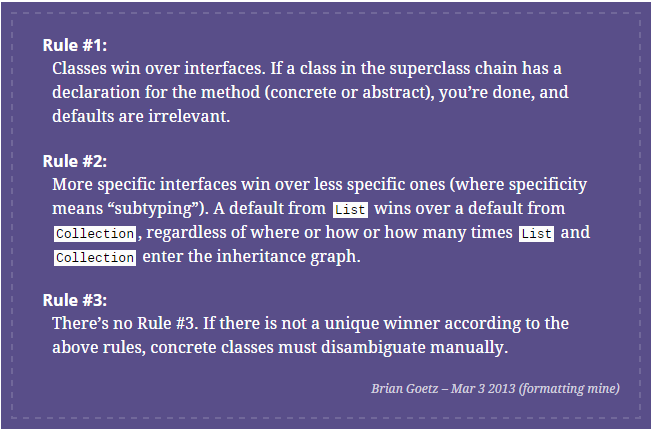
\includegraphics[width=5in]{screenshot.png}
\caption{Screenshot.}\label{screenshot_png}
\end{figure}

\haoyuan{I tried to understand the current algorithm, and did more experiments in eclipse.
Now I borrow some ideas from the current version, and give a new version of the algorithm in text. See below.

(1) I guess the function \textsf{tops} is not necessary. The first step is still
\[\textsf{mbody}(m,C_i)\in\overline{meth}\textrm{ (excluding \textbf{static} methods)}\]

(2) Assume the context is ``interface $C_0$ extends $\overline{C}$ \{$meth'$;...\}''. First handle
\[\textsf{override}(meth',\overline{meth}) \eqno{(*)}\]

(3) If $meth'\ne\none$, $(*)$ returns $meth'$ if
\[\forall meth\in\overline{meth},meth'\subtype meth\]
even if there are conflicts in $\overline{meth}$.

(4) If $meth'=\none$, we need to figure out
\[\textsf{mostSpecific}(\overline{meth})\]
and it should be the one that ``overrides'' all the others in $\overline{meth}$. It means we should not only deal with the return types of methods, but also look into the subtyping relation of interfaces. But for abstract methods, only return types are taken into consideration.
}
\end{comment}

%\text{\yanlin{shouldn't mostSpecific be: $\forall \method' \in \methods : \method \subtype
%  \method'$ ?}}

%(2) If $body_1.\textsf{returnType}=body_2.\textsf{returnType}$, \textsf{shadow} tends to return a default method. If both $body_1$ and $body_2$ are default methods, \textsf{shadow} throws an error.
%\begin{equation*}
%\begin{array}{ll}
%\textsf{shadow}(body_1, body_2)=\textsf{ERROR} & \textsf{if }body_1.\textsf{modifier}=body_2.\textsf{modifier}=\textbf{default}\\
%\textsf{shadow}(body_1, body_2)=body_1 \hspace{.1in} & \textsf{if }body_1.\textsf{modifier}=\textbf{default} \\
%\textsf{shadow}(body_1, body_2)=body_2 \hspace{.1in} & \textsf{if }body_2.\textsf{modifier}=\textbf{default} \\
%\textsf{shadow}(body_1, body_2)=body_1\textsf{ (or }body_2\textsf{)} \hspace{.1in} & \textsf{otherwise}
%\end{array}
%\end{equation*}
%
%(3) If $body_1.\textsf{returnType}<:body_2.\textsf{returnType}$, \textsf{shadow} tends to choose the one with the subtype (namely $body_1$), but only when both methods are abstract, otherwise it gives an error. The other direction $body_2.\textsf{returnType}<:body_1.\textsf{returnType}$ follows the same rule. It also gives an error if there is no subtyping relationship between two return types.
%\begin{equation*}
%\begin{array}{ll}
%\textsf{shadow}(body_1, body_2)=body_1 & \textsf{if }body_1.\textsf{modifier}=body_2.\textsf{modifier}=\emptyset\\
%& \textsf{and }body_1.\textsf{returnType}<:body_2.\textsf{returnType}\\
%\textsf{shadow}(body_1, body_2)=body_2 & \textsf{if }body_1.\textsf{modifier}=body_2.\textsf{modifier}=\emptyset\\
%& \textsf{and }body_2.\textsf{returnType}<:body_1.\textsf{returnType}\\
%\textsf{shadow}(body_1, body_2)=\textsf{ERROR} \hspace{.1in} & \textsf{otherwise}
%\end{array}
%\end{equation*}

%\subsubsection{Auxiliary function: \textsf{replace}}
%
%The \textsf{replace} function takes two same methods (with the same name and types of arguments), and gives the result of the first method overriding the second one.
%
%\begin{equation*}
%\begin{array}{ll}
%\textsf{replace}(body_1, body_2)=body_1 & \textsf{if }body_2=\emptyset\\
%\textsf{replace}(body_1, body_2)=body_2 & \textsf{if }body_1=\emptyset\\
%\textsf{replace}(body_1, body_2)=body_1 & \textsf{if }body_1.\textsf{returnType}<:body_2.\textsf{returnType}\\
%\textsf{replace}(body_1, body_2)=\textsf{ERROR} \hspace{.1in} & \textsf{otherwise}
%\end{array}
%\end{equation*}
